%!TEX root = ../report.tex
\documentclass[report.tex]{subfiles}
\begin{document}
    \chapter{Introduction}
    % \begin{itemize}
    %     \item Imagine driving on a winding mountain road at night, with fog and rain obscuring your view, your vehicle's self-driving system struggles to detect objects ahead due to the challenging weather conditions. Suddenly, a deer jumps out in front of your car, causing the system to issue an alert and apply the brakes in time to avoid a collision.

    %     \item This scenario highlights the importance of object detection in adverse weather conditions for self-driving cars. Visual cameras, which are commonly used for object detection, may be distorted or obscured by rain, fog, snow, or low light, making it difficult to accurately detect objects on the road \cite{yurtsever2020survey} \cite{carballo2020libre} \cite{mcity2020}.
        
    %         \begin{figure}[h]
    %             \centering
    %             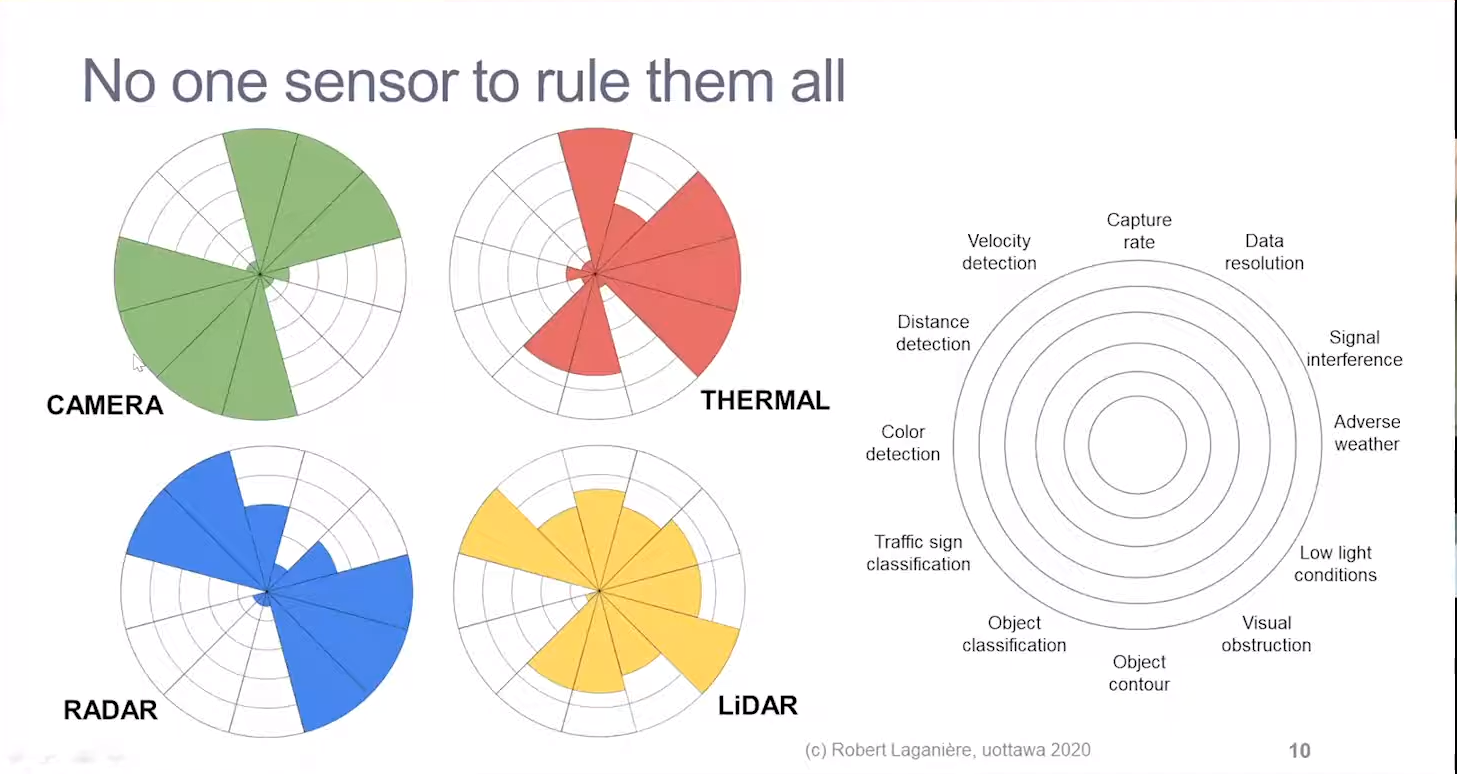
\includegraphics[width=0.7\textwidth]{images/sensors_intro_1.png}
    %             \caption{Sensors modality characteristics \cite{Sensor_modality_characteristics_1}}
    %             \label{fig:sensors_intro_1}
    %         \end{figure}

    %     \item The Figure \ref{fig:sensors_intro_1} outlines the strengths and challenges of different sensors used in automated systems, based on work by Robert \cite{Sensor_modality_characteristics_1}. It compares how well cameras, thermal sensors, radars, and LiDARs perform in various conditions. Cameras are good at recognizing colors and signs but not as effective in the dark or measuring distance. Thermal sensors perform well in bad weather but can't detect colors or missing texture information. Radars are great for measuring speed and aren’t affected by things blocking their view, but their data points are sparse and noisy. LiDAR sensors are excellent at mapping the shape and size of objects and unaffected in low light conditions, but their performance drops in poor weather. This comparison shows why combining these sensors is a smart approach to improve safety and reliability in automated driving systems, as it allows each sensor to cover the gaps of the others. The Figure \ref{fig:sensors_intro_2} exemplifies fusion of complementary sensors in order to achieve complete understanding of the environment.
        
    %     \item To address these challenges, this project aims to implement a multimodal sensor fusion system that combines cameras, radar, and LiDAR sensors. By fusing data from multiple sensors and leveraging advanced machine learning algorithms, the goal is to enhance object detection's range, accuracy, and reliability in adverse weather conditions.
        
    %     \item The focus will also be on synchronizing multimodal data, processing dense and sparse resolution sensor data, and using a data-driven approach to optimize object detection performance.

    %         \begin{figure}[h]
    %             \centering
    %             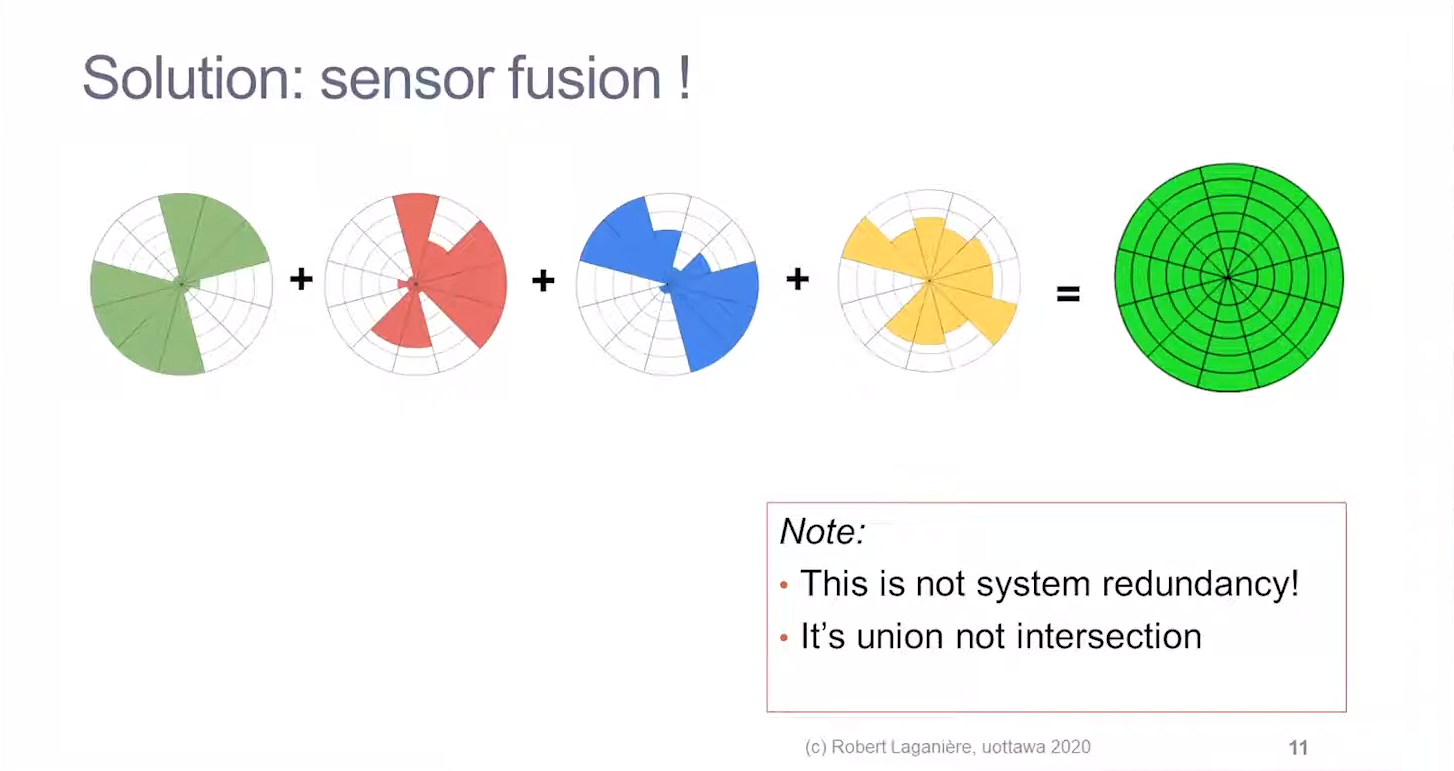
\includegraphics[width=0.7\textwidth]{images/sensors_intro_2.png}
    %             \caption{Sensors modality characteristics \cite{Sensor_modality_characteristics_1}}
    %             \label{fig:sensors_intro_2}
    %         \end{figure}

    %     \item However, this project also faces several challenges. For example, different sensors may have different resolutions, sampling rates, and may require sophisticated calibration and alignment techniques to ensure the accurate fusion of their data. Furthermore, processing large volumes of sensor data with minimal latency requires efficient and scalable algorithms and hardware architectures.

    %     \item The proposed system will be trained on a diverse dataset to ensure robustness and adaptability in different weather and lighting conditions. The system's effectiveness will be evaluated by extensive experiments and by comparing existing state-of-the-art methods.

    %     \item Despite the challenges, the project has the potential to revolutionize object detection in adverse weather conditions, with applications ranging from self-driving cars, drones to surveillance, and security systems. By fusing multiple sensor data sources and optimizing their fusion, situational awareness can be enhanced, enabling safer and more efficient operations in various domains.

    %     \item This research aims to facilitate safe and efficient self-driving in adverse weather conditions, prioritizing the safety of passengers, other drivers, and pedestrians on the road. To accomplish this, the proposed approach is to develop a sensor fusion system that operates with minimal latency, enabling data processing from multiple sensors in near real-time.
    %     \item Topic naming convention:
    %       \begin{itemize}
    %           \item Object detection
    %                 \begin{itemize}
    %                     \item Refers to the task of detecting objects within an image or video stream.
    %                     \item In this project, the focus is on detecting objects such as cars, trucks, pedestrians, and cyclists.
    %                 \end{itemize}
    %           \item Adverse weather conditions
    %                 \begin{itemize}
    %                     \item Refers to conditions such as fog, snow, rain, overcast skies, sleet, and dust.
    %                     \item These conditions can make object detection more challenging due to reduced visibility or other environmental factors.
    %                 \end{itemize}
    %           \item Tightly-coupled
    %                 \begin{itemize}
    %                     \item Refers to how different modalities of data are combined and integrated at different levels.
    %                     \item Rather than relying solely on early, mid, or late fusion techniques, a combination of features at different levels is employed to achieve optimal fusion results.
    %                 \end{itemize}
    %           \item Data-driven
    %                 \begin{itemize}
    %                     \item Refers to the use of previously collected data or publicly available datasets to improve object detection performance.
    %                 \end{itemize}
    %           \item Multimodal
    %                 \begin{itemize}
    %                     \item Refers to the use of different data modalities to improve object detection performance.
    %                     \item Examples include sensors such as camera, LIDAR, RADAR, IMU, GPS, and infrared, with different datatypes such as point clouds, images, and time series data.
    %                 \end{itemize}
    %           \item Sensor fusion
    %                 \begin{itemize}
    %                     \item Refers to the process of fusing data from different sensors to get a better estimation of an environment and improve object detection performance.
    %                 \end{itemize}
    %       \end{itemize}
    % \end{itemize}


        In the realm of autonomous driving, the ability to detect objects in challenging weather conditions remains a critical area of research. Consider a scenario where a self-driving vehicle navigates a winding mountain road at night amidst fog and rain. The limitations of the vehicle's visual cameras become evident as they struggle to detect objects due to reduced visibility, highlighting the crucial need for advanced object detection methods in adverse weather conditions. This is particularly significant in emergency situations, like when a deer suddenly appears on the road, necessitating quick and accurate object detection to prevent accidents \cite{yurtsever2020survey} \cite{carballo2020libre} \cite{mcity2020}.

        As depicted in Figure \ref{fig:sensors_intro_1}, the performance of various sensors in automated systems under different conditions has been extensively analyzed. Cameras, for instance, excel in recognizing colors and signs but falter in dark or distant object measurement. Conversely, thermal sensors maintain efficiency in poor weather but lack color detection and texture information. Radar sensors are adept at speed measurement and are less hindered by visual obstructions, though they produce sparse and noisy data. LiDAR sensors, meanwhile, provide excellent object shape and size mapping but underperform in poor weather conditions \cite{Sensor_modality_characteristics_1}.

        \begin{figure}[h]
            \centering
            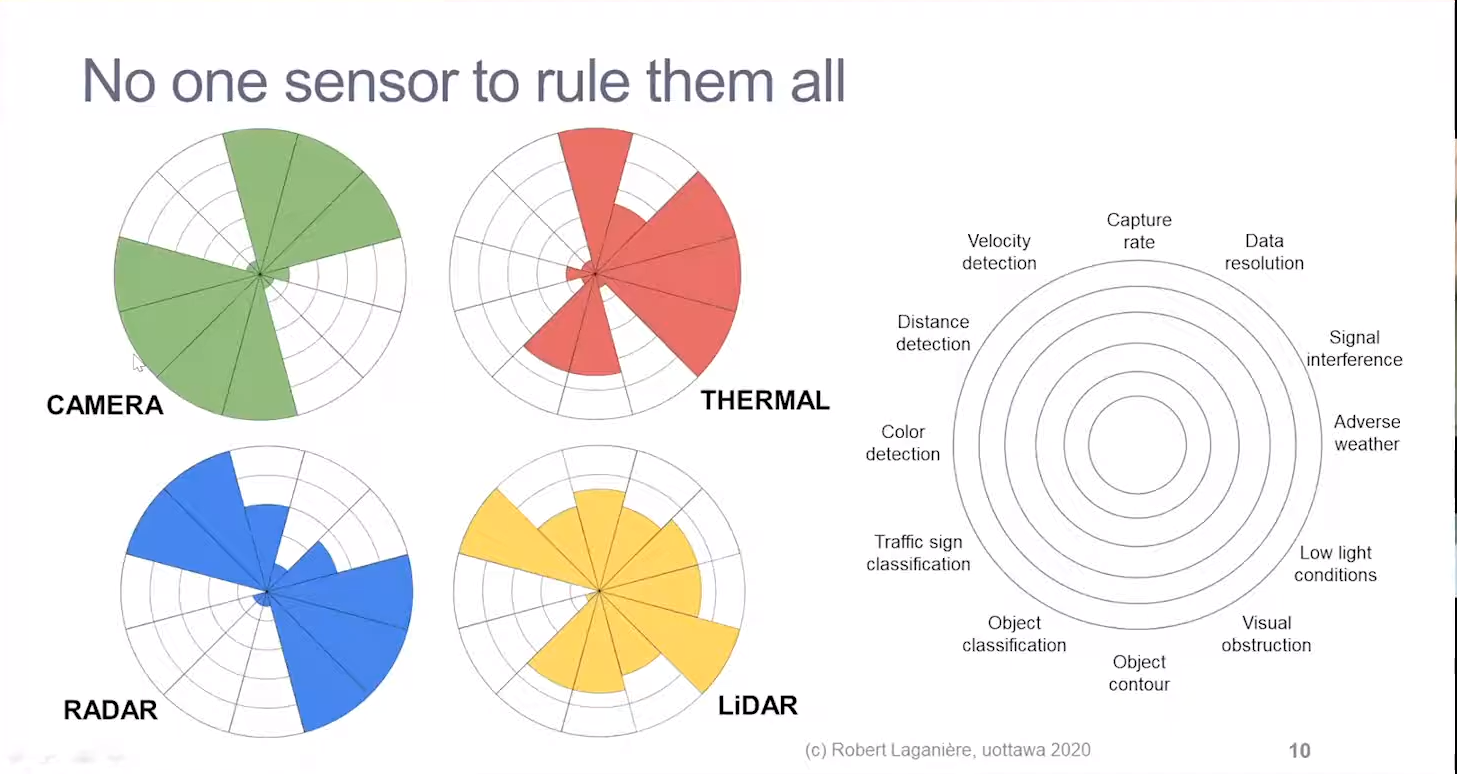
\includegraphics[width=0.7\textwidth]{images/sensors_intro_1.png}
            \caption{Sensors modality characteristics \cite{Sensor_modality_characteristics_1}}
            \label{fig:sensors_intro_1}
        \end{figure}

        To overcome these limitations, this project proposes the development of a tightly-coupled multimodal sensor fusion system, as exemplified in Figure \ref{fig:sensors_intro_2}. By integrating cameras, radar, and LiDAR sensors, this approach harnesses the unique strengths of each to create a comprehensive and reliable object detection framework. The fusion of these complementary sensors, coupled with advanced machine learning algorithms, aims to significantly enhance the range, accuracy, and reliability of detection in adverse weather conditions. Effectively synthesizing diverse data sources enables the creation of a robust and responsive system that overcomes the weaknesses of any individual sensor type.

        \begin{figure}[h]
            \centering
            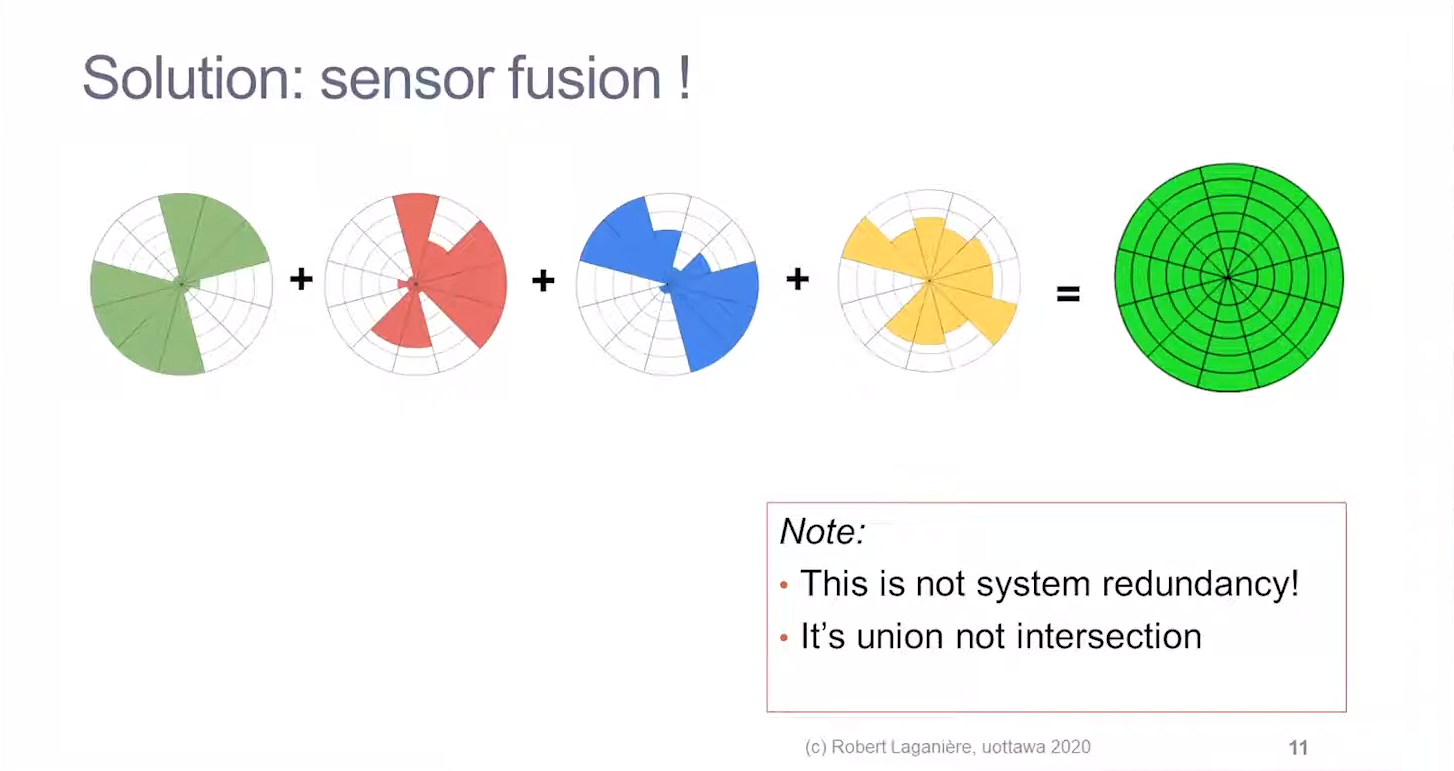
\includegraphics[width=0.7\textwidth]{images/sensors_intro_2.png}
            \caption{Sensors modality characteristics \cite{Sensor_modality_characteristics_1}}
            \label{fig:sensors_intro_2}
        \end{figure}

        However, the integration of different sensor types presents its own set of challenges, such as varying resolutions, sampling rates, and the need for sophisticated calibration and alignment techniques. These hurdles necessitate the development of efficient and scalable algorithms and hardware architectures capable of processing large volumes of sensor data with minimal latency.

        Despite these challenges, the anticipated outcomes of this project are transformative, with potential applications extending beyond autonomous vehicles to drones, surveillance, and security systems. By enhancing situational awareness through optimized sensor fusion, the project aims to foster safer and more efficient operations across various sectors. The primary objective is to ensure safe and efficient autonomous driving in adverse weather conditions, prioritizing the safety of passengers, other drivers, and pedestrians. This will be achieved through a sensor fusion system designed for minimal latency, enabling the processing of data from multiple sensors in near real-time.

        % The project will also delve into specific aspects of object detection, such as identifying various entities like cars, trucks, pedestrians, and cyclists, and will focus on detection in adverse weather conditions like fog, snow, and rain, which pose significant challenges to visibility. The 'tightly-coupled' approach refers to the intricate integration of different data modalities, combining features at various levels for optimal results. The 'data-driven' aspect emphasizes leveraging existing datasets to enhance performance, while 'multimodal' pertains to the utilization of diverse sensor types. Finally, 'sensor fusion' is central to the project, entailing the amalgamation of data from different sensors to improve environmental perception and object detection capabilities.

        In this research, the focus is specifically on 2D object detection to manage the intricacies of network and computational complexity. This scope simplifies the task of handling high-dimensional data, allowing for a more streamlined implementation while addressing the challenge of object detection in adverse weather conditions. Such conditions, including fog, snow, and rain, significantly hinder the visibility and recognition of various entities like cars, trucks, pedestrians, and cyclists. The 'tightly-coupled' approach involves the intricate integration of various data modalities, combining features at multiple levels for optimal results. The 'data-driven' aspect emphasizes leveraging existing datasets to enhance performance, while 'multimodal' pertains to the utilization of diverse sensor types. Finally, 'sensor fusion' is central to the project, entailing the amalgamation of data from different sensors to improve environmental perception and object detection capabilities.
    
    % \section{Relevance}

    % \begin{itemize}

    %     \item The relevance of the research project lies in the fact that weather phenomena have a significant negative influence on traffic and transportation, which can lead to accidents, injuries, and fatalities.

    %     \item The statistics show that adverse weather conditions, such as rain, snow, sleet, and fog, contribute to a high number of vehicle crashes and fatalities worldwide.

    %     \item For example, in the United States, over 30,000 vehicle crashes occur on snowy or icy roads each year, causing over 5,000 fatalities and 418,000 injuries due to adverse weather-related crashes, according to the Federal Highway Administration (FHA) \cite{federal-highway-administration-no-date} \cite{usDepartmentofCommerce2016}.

    %     \item According to a study by the Insurance Institute for Highway Safety (IIHS), the likelihood of fatal crashes increases significantly during snowy weather conditions, with a 21\% higher rate compared to clear roads. The rate is even higher at 37\% during sleet and freezing rain. Furthermore, a report by the National Highway Traffic Safety Administration (NHTSA) in 2018 revealed that adverse weather conditions were involved in 4,000 fatal crashes \cite{brumbelow2022light}.

    %     \item In Europe, adverse weather conditions cause 25\% of all road accidents, with frost and ice, snow, and rain being the highest contributing factors, according to the European Commission and the European Transport Safety Council (ETSC). Over 12,000 people die on European roads each year in weather-related accidents \cite{cookson-2022}.

    %     \item Furthermore, the project's results will benefit various sectors, including autonomous vehicles, healthcare, precision agriculture, environmental monitoring, aerospace and defense, and industrial automation.
        
    %     \item In 2019, the global market for sensor fusion used in autonomous vehicles had a value of USD 594.4 million. According to estimates, this market is expected to grow significantly and reach a value of USD 1563.5 million by 2025, reflecting a Compound Annual Growth Rate (CAGR) of 19.6\% during the period between 2020 and 2025. According to MarketInsider, autonomous emergency braking (AEB) is expected to drive significant growth in the use of sensor fusion, as AEB systems rely on radar and vision sensors to identify potential collision partners ahead of the ego vehicle. North America is predicted to be one of the largest markets for ADAS-enabled vehicles and self-driven transport solutions \cite{marketInsider}.

    %     \item In the healthcare sector, wearable sensors are estimated to reach over \$1.5 billion in revenue by 2030, growing at a CAGR of over 18.3\% \cite{straitsresearch2021}.

    %     \item For precision agriculture and environmental monitoring, the market is expected to reach \$10.5 billion by 2026, growing at a CAGR of over 12.6\% \cite{mordorintelligence2023}.

    %     \item The aerospace and defense sector, including aircraft navigation and control, missile guidance, and military logistics, is expected to reach \$23.83 billion by 2027, at a CAGR of 4.21\% \cite{fortunebusinessinsights2023}.

    %     \item Even the industrial automation sector benefits from the sensor fusion technology as it can improve the efficiency of the production process and reduce the cost of production.
        
    % \end{itemize}
    
    \section{Motivation}

        The motivation for the research topic is deeply rooted in the understanding that weather phenomena significantly impact traffic and transportation safety. Adverse weather conditions, such as rain, snow, sleet, and fog, are major contributors to the high number of vehicle crashes and fatalities worldwide. This problem is particularly acute in regions with severe weather variations.

        In the United States, over 30,000 vehicle crashes occur annually on snowy or icy roads, resulting in over 5,000 fatalities and 418,000 injuries, as reported by the Federal Highway Administration \cite{federal-highway-administration-no-date} and the US Department of Commerce \cite{usDepartmentofCommerce2016}. The Insurance Institute for Highway Safety (IIHS) underscores this issue, noting that the likelihood of fatal crashes increases by 21\% during snowy weather conditions, primarily due to reduced visibility, compared to clear roads. It has been proven that the risk of accident in rain conditions is 70\% higher than normal \cite{andrey1993temporal}. A 2018 report by the National Highway Traffic Safety Administration (NHTSA) further underscores that adverse weather conditions were involved in 4,000 fatal crashes \cite{brumbelow2022light}.
        
        In Europe, adverse weather conditions are responsible for 25\% of all road accidents. Frost, ice, snow, and rain significantly reduce drivers' perceptible range from hundreds of meters to just a few meters, leading to over 12,000 fatalities annually on European roads due to weather-related accidents, as indicated by the European Commission and the European Transport Safety Council (ETSC) \cite{cookson-2022}. This drastic reduction in visibility poses a major challenge for effective obstacle or object detection, a critical component of road safety in adverse conditions.

        In the context of current advancements in autonomous vehicles (AVs), a persistent challenge remains their operation in inclement weather conditions such as heavy rain or snow, which raises safety concerns. Extensive research and trials have been conducted under adverse weather conditions, yet the Mcity shuttle, for instance, ceases operation when continuous use of windshield wipers is necessitated in rain or snow \cite{briefs2015mcity}. Tesla's autopilot system exhibits a limited capability to navigate through mild rain or snow, provided road markings are visible, but encounters difficulties in more severe conditions like heavy storms or obscured lane lines \cite{Lambert2019}. Similarly, General Motors' Super Cruise, another prominent Level 2 autonomous driving system, explicitly restricts the use of its self-driving function in hazardous conditions, including rain, sleet, fog, ice, or snow \cite{cadillac2021supercruise}. These limitations indicate that, despite advancements, autonomous vehicles are not yet reliable enough to operate independently of human drivers in all weather conditions. Consequently, overcoming these environmental constraints is imperative for the advancement of autonomous driving systems (ADS) into a new era of complete autonomy.
        
        The relevance of this research extends beyond road safety, impacting sectors such as autonomous vehicles, healthcare, precision agriculture, environmental monitoring, aerospace, defense, and industrial automation. For instance, the market for sensor fusion in autonomous vehicles, vital for enhancing object detection capabilities under adverse weather conditions, was valued at USD 594.4 million in 2019. It is projected to grow to USD 1563.5 million by 2025, according to MarketInsider \cite{marketInsider}. This growth reflects the increasing reliance on advanced sensor technologies, such as radar and vision sensors, for autonomous emergency braking (AEB) systems and other ADAS applications.
        
        Similarly, In the healthcare sector, the market for wearable sensors, which typically integrate multiple sensors for comprehensive health data, is expected to reach over \$1.5 billion by 2030 \cite{straitsresearch2021}. The precision agriculture and environmental monitoring markets are anticipated to reach \$10.5 billion by 2026 \cite{mordorintelligence2023}, while the aerospace and defense sector is projected to reach \$23.83 billion by 2027 \cite{fortunebusinessinsights2023}. Each of these sectors can benefit significantly from advancements in sensor fusion technology, enhancing efficiency and reducing production costs in industrial automation.
        
        The focus of this research on developing and applying data-driven multimodal sensor fusion techniques for object detection in adverse weather conditions is vital not only for improving road safety in autonomous vehicles but also holds the potential to revolutionize various technology-driven sectors. By addressing the challenges of object detection in complex and unpredictable weather conditions, this research aims to contribute significantly to the fields of autonomous vehicles, healthcare, environmental monitoring, and beyond.

    \section{Challenges and Difficulties}

        The field of multimodal sensor fusion, particularly in the context of adverse weather conditions, presents a series of distinct challenges that are critical to the advancement of reliable object detection systems. These challenges range from the scarcity of specialized datasets to the intricacies of fusion architecture, computational demands, and the search for effective network design and generalization. This section outlines the key challenges in this field.

        \textbf{Scarcity of Adverse Weather-Related Datasets}: A fundamental challenge in this field is the lack of datasets that capture adverse weather conditions through multimodal sensors. Most existing datasets are oriented towards clear weather scenarios. For example, popular datasets for multimodal sensor fusion include camera and LiDAR but often lack radar sensors. These include KITTI \cite{geiger2012we}, ApolloScape \cite{huang2019apolloscape}, and Waymo \cite{sun2020scalability}. There are datasets that incorporate radar sensors, such as VoD \cite{palffy2022multi}, TJ4DRadSet \cite{zheng2022tj4dradset}, and PixSet \cite{deziel2021pixset}, but they do not cover an extensive range of adverse weather conditions. This limitation restricts the development and validation of object detection models in more challenging environmental conditions and hinders the advancement of robust object detection systems capable of performing reliably under diverse weather conditions.

        \textbf{Limitations in Fusion Architecture}: The predominant focus in the current landscape of fusion architectures is on middle or feature fusion, with only limited exploration in the area of tightly coupled fusion networks. This trend poses a particular challenge for sensor fusion that involves radar data, which tends to be noisier and sparser compared to the data produced by cameras and LiDAR. The scarcity of research on tightly coupled fusion methods for integrating such diverse data types is a significant obstacle in developing efficient and effective multimodal fusion systems.

        \textbf{Computational Constraints}: Another significant barrier is the computational demand required to train large, complex networks. This requirement often exceeds the resources available to many researchers, restricting exploration in this field and slowing the advancement of more sophisticated fusion methods.

        \textbf{General Guidelines for Network Architecture}: Currently, there is no standard or widely accepted framework for the design of network architectures in multimodal sensor fusion, leading to several unanswered questions. Key considerations, as highlighted by Feng et al. \cite{feng2020deep}, include:
        \begin{itemize}
            \item "What to fuse," such as LiDAR, radar, various camera types (color, thermal, event), or ultrasonic sensors;
            \item "How to fuse," with possibilities including addition or averaging, concatenation;
            \item "When to fuse," which can range from early, mid, late, or a combination of these fusion stages.
        \end{itemize}
        This absence of a clear guideline results in uncertainties regarding the optimal choices for integrating different modalities in sensor fusion.

        \textbf{Limited Generalization from Previous Studies}: Many existing studies in multimodal sensor fusion have focused on results from their baseline models and custom datasets. This narrow scope limits the generalizability of their findings, as these models may not perform as well under different conditions or with alternative datasets.

        \textbf{Advanced Fusion Methods and Temporal Information}: While recent datasets have begun to include baseline models featuring basic fusion methods, there is notable potential for significant performance enhancement. This can be achieved by incorporating advanced transformer-based architectures, known for their superior handling of complex data patterns and scalability. Additionally, employing sophisticated fusion techniques, such as tightly-coupled fusion, which integrates data more closely and efficiently, could further optimize the sensor fusion process. Additionally, the integration of temporal information in sensor fusion is an area that is yet to be extensively explored. Although not a focus of this project, it represents a promising direction for future research.

        Addressing these challenges is critical for advancing the field of object detection in adverse weather conditions using multimodal sensor fusion. This research will contribute to this effort by exploring these underdeveloped areas, aiming to find more robust and effective object detection systems.

    \section{Problem Statement}
    % \begin{itemize}
    %     \item Object detection using multiple modalities has become a topic of increasing interest in recent years. However, despite the wealth of research in this area, there is still a lack of comprehensive analysis and practical implementation of state-of-the-art methods under adverse weather conditions. Therefore, the primary objective of this research project is to provide a thorough analysis and practical implementation of state-of-the-art methods for object detection using multiple modalities, including but not limited to camera, LiDAR, and radar.

    %     \item One of the significant challenges in multimodal object detection is determining an appropriate fusion strategy to exploit the complementary characteristics of various sensors. For instance, fusing camera and 4D radar data is a critical research question that needs to be addressed. This research project will focus on identifying an optimal fusion strategy that leverages the strengths of each sensor while minimizing their weaknesses.
        
    %     \item This research project aims to conduct experiments to evaluate the performance of the proposed methods under adverse weather conditions. To achieve this, the outcomes will be compared with various models on publicly available datasets such as DENSE \cite{bijelic2020seeing}, and nuScenes \cite{caesar2020nuscenes}. These datasets are deemed suitable for the purpose of analyzing the performance of the proposed methods under challenging conditions.
      
    %     \item The comparative analysis of the results will include an assessment of the strengths and weaknesses of each approach with respect to existing state-of-the-art methods.        

    % \end{itemize}

    The field of object detection using multiple modalities has become a topic of increasing interest in recent years, reflecting the growing demand for advanced sensing technologies in various applications, especially in autonomous vehicles and robotics. However, the comprehensive analysis and practical application of state-of-the-art multimodal object detection methods under adverse weather conditions remain largely unexplored areas. The crux of this research project is to bridge this gap by providing an in-depth analysis and practical implementation of cutting-edge techniques in multimodal object detection. The project will explore the integration of multiple sensor modalities, including but not limited to cameras, LiDAR, and radar, to enhance detection capabilities in challenging weather scenarios.

    One key aspect of this project is its focus on 2D object detection, a deliberate choice to reduce the complexities associated with network and computer processing. While simplifying the technical challenges, this focus does not diminish the project's primary objective: to explore object detection in adverse weather conditions through a multimodal approach and tightly coupled fusion architecture.
    
    A pivotal challenge in this field is exploring an effective fusion strategy that capitalizes on the complementary strengths of different sensors while mitigating their individual limitations. For example, the integration of visual camera data with radar information presents a complex yet crucial research question. This research aims to explore an optimal fusion strategy, a technique that effectively combines the unique strengths of each sensor type, thereby creating a more robust and accurate detection system. The strategic combination of these modalities holds the potential to significantly enhance object detection performance, especially in conditions where traditional single-sensor systems fall short.

    To empirically validate the effectiveness of the proposed methods, this project will conduct comprehensive experiments under a variety of adverse weather conditions. The performance of these methods will be rigorously tested and compared using renowned publicly available datasets, such as DENSE \cite{bijelic2020seeing} and nuScenes \cite{caesar2020nuscenes}. These datasets, known for their suitability in evaluating performance under challenging environmental conditions, will serve as the benchmark for assessing the robustness and reliability of the proposed multimodal object detection techniques.

    Additionally, this study will compare the proposed methods to the best existing methods by comparing their outcomes. This comparison will not only highlight the efficacy of the new methods in adverse conditions but will also shed light on the strengths and weaknesses of each approach. Through this evaluation, the project aims to contribute significantly to the body of knowledge in multimodal object detection, providing valuable insights for future research and practical applications in this rapidly evolving field.

    % \subsection{...}

    % \lipsum[21-30]

    % \subsection{...}


    % \subsection{...}
\end{document}
